\chapter{Werkzeuggestützte Analyse}


\section{Lernziele}

\begin{itemize}
    \item für kleinere Projekte qualitätssichernde Maßnahmen planen und verfolgen können
    \item Tests planen und dokumentieren können
    \item gefundene Fehler geeignet verwalten können
\end{itemize}

\newpage

\section{Einleitung}

Viele Produkte der Softwareentwicklung (\textit{Artefakte}) sind nicht testbar, dazu gehören bspw. Dokumente, die Anwendungsfälle beschreiben, das Data Dictionary\footnote{
hält fest, in welchem Format welche Daten verarbeitet werden
} aber auch Klassendiagramme aus Analyse und Entwurf.\\
Wenn sich die Qualität von Artefakten nicht oder nicht ausschließlich durch Testen sicherstellen lässt, kommen \textbf{manuelle Verfahren} zum Einsatz: Mitarbeiter untersuchen den \textbf{Prüfgegenstand} durch \textbf{systematisches Korrekturlesen}.\\

\noindent
Es ist wichtig, Defekte früh im Entwicklungsprozess zu finden.\\
Bei einem falschen Entwurf oder einer falschen Spezifikation fällt der Fehler u.U. erst in eienr späten Phase bei den \textbf{Systemtests} durch spezialisierte Tester\footnote{
s. Abschnitt~\ref{sec:v-modell}
} oder bei dem \textbtf{Abnahmetest} durch den Kunden auf.\\
Fehlerhafter Code kann also auch in frühen Phasen durch das \textbf{manuelle Prüfen} von Dokumenten und Modellen verhindert werden, indem andere Personen Prüfgegenstände \textit{systematisch lesen}.\\
Hierbei kommen auch \textbf{Checklisten} zum Einsatz.\\
Gefundene Defekte und Verbesserungsvorschläge werden dem \textbf{Autor} vom \textbf{Prüfer} mitgeteilt.\\

\noindent
Die Funktionsfähigkeit von Software wird i.d.R. durch Tests sichergestellt, aber auch eine manuelle Prüfung kann sinnvoll sein: Manche Defekttypen werden so effektiver gefunden\footnote{
das \textit{Vieraugenprinzip} gilt als effektive präventive Kontrolle, s. \url{https://de.wikipedia.org/wiki/Vier-Augen-Prinzip}, abgerufen 22.05.2024
}.
Außerdem kann nur bei einer Analyse des Quellcodes überprüft werden, ob ein Entwickler den Quellcode auf eine \textbf{wartbare} Art und Weise geschrieben hat, also ob der Code \textbf{lesbar} und \textbf{einfach zu ändern} ist\footnote{
dass die Einhaltung von Coding-Standards im gesamten Quellcode besser automatisierte durch Werkzeuge stattfindet, bleibt hiervon unberührt
}.\\

\noindent
Ein wichtiger Nebeneffekt manueller Prüfverfahren ist, dass sich der Prüfer \textit{intensiv} mit dem Prüfgegenstand \textit{auseinandersetzt}.
Dies wirkt sich positiv bei einem Ausfall oder einer Umstrukturierung aus.\\

\noindent
Manuelle Prüfungen sind recht aufwändig, was sich auch in den Kosten widerspiegelt.
Aus diesem Grund schrecken viele Projektverantwortliche davor zurück. \textit{Wedemann} führt an, dass im Zuge einer \textit{objektiven Argumentation} die Kosten miteinander verglichen werden sollten, die bei der Beseitigung der Defekte in bestimmten Phasen entstehen (vgl.~\cite[16]{Wed09c}).
Auch \textit{Brooks} weist auf die Notwendigkeit hin, Defekte möglichst früh zu erkennen:

\blockquote[{\cite[142]{Bro95}}]{
The most pernicious and subtle bugs are system bugs arising from mismatched assumptions made by the authors or various components. [\ldots] Long before any code exists, the specification must be handed to an outside testing group to be scrutinized for completeness and clarity.
}

\noindent
\textit{Wedemann} schließt aus verschiedenen Quellen (\cite{Rad01}, \cite{Wie02}, \cite{GG93}), dass eine Reduktion der Kosten zur Behebung von Defekten erreicht werden kann, wenn diese Defekte bei einer manuellen Überprüfung in einer frühen Phase gefunden werden.
Weiter stellt er fest,  dass ``bei einer Inspektion ca. 60{\%} aller Defekte gefunden werden`` (~\cite[16]{Wed09c}).\\

\noindent
Prinzipiell sollten alle Dokumente und Modelle mit manuellen Verfahren geprüft werden, da diese Verfahren das einzig praktikable Verfahren sind (\cite[16]{Wed09c}).\\
Manuell geprüft werden sollten insb.

\begin{itemize}
    \item wichtige Codeteile:
    \begin{itemize}
        \item \textbf{Vorlagen}
        \item denen eine \textbf{entscheidende Rolle} in der Software zukommt
    \end{itemize}
    \item Code, der von \textbf{neuen} oder \textbf{unerfahrenen Mitarbeitern} geschrieben wird
\end{itemize}

\noindent
Der Einsatz von manuellen Verfahren ist unkompliziert, allerdings sollte vor Beginn der Entwicklung überlegt werden, welche manuellen Verfahren durchgeführt werden sollen.
Diese Abläufe sollten im Management-Plan schriftlich fixiert werden, um das Verständnis aller Mitarbeiter zu schärfen.
Es sollte außerdem ausreichend Zeit zur Durchführung der Maßnahmen eingeplant werden und die Durchführung dementsprechend verfolgt und die Ergebnisse protokolliert werden.\\
Wenn Autoren die Maßnahmen als unangenehm empfinden, sollte bei der Durchführung sorgsam mit ihnen umgegangen werden (vgl. \cite[17]{Wed09c}).
\section{Programmierrichtlinien}\label{sec:programmierrichtlinien}

\subsection*{Einhaltung der Programmierrichtlinien wichtig für Wartbarkeit}

Die \textbf{Einhaltung von Programmierrichtlinien} ist eine naheliegende Aufgabe für die \textbf{werkzeuggestützte Analyse}.\\
\textbf{Programmierrichtlinien} können \textbf{projektweit}, \textbf{unternehmensweit} oder \textbf{weltweit} (wie bei Java\footnote{
s. \url{https://www.oracle.com/java/technologies/javase/codeconventions-introduction.html}, abgerufen 24.05.2024
}) vorgegeben sein.\\

\noindent
Die Einhaltung von Programmierrichtlinien ist wichtig für die \textbf{Qualitätsforderung} \textbf{Wartbarkeit}: \textbf{Wartbarkeit} setzt auch voraus, dass der Code verständlich und damit einfach lesbar ist.

\subsection*{Ursachen für gefundene Defekte}
Ein erster Einsatz solcher Werkzeuge ist meist sehr ernüchternd: Oft werden mehr Defekte angezeigt, als praktischerweise behoben werden können.
Die hängt u.a. damit zusammen, dass

\begin{enumerate}
    \item die Einstellungen der IDE meistens nicht mit der Einstellung der Analysewerkzeuge zusammenpassen
    \item viele Entwickler die Programmierrichtlinien nicht gut genug kennen
    \item manche der standardmäßig vorgegebenen Programmierrichtlinien für die Praxis zu strikt sind
\end{enumerate}

\noindent
Bei existierendem Code sind \textit{nachträgliche} Programmierrichtlinien schwer durchzusetzen.
Es ist denkbar, in solchen Fällen die Programmierrichtlinien nur für neuen Code durchzusetzen.

\subsection*{Vorgehen}
\begin{itemize}
    \item Werkzeuge sollten von Anfang an benutzt werden, da ein nachträglicher Einsatz mit hohem Aufwand verbunden ist.
    \item Die Einführung sollte zunächst an einem kleinen Stück Software erprobt werden, die Einstellungen der IDE werden dann anhand des Beispiels angepaßt, Regeln ggf. modifiziert
    \item während des ersten Gebrauchs sollten die Regeln systematisch auf die Brauchbarkeit überprüft und Werkzeug und IDE  angepaßt werden, bis ein akzeptabler Stand erreicht ist
    \item die Projektleitung sollte darauf achten, dass alle Entwickler den Quellcode gleich prüfen - das Werkzeug sollte also in die IDE integriert sein, zumindest aber in das Build-Management, damit die Prüfung automatisch und periodisch durchgeführt wird
\end{itemize}

\subsection*{Werkzeuge}
Für Java gibt es für die Einhaltung von Programmierrichtlinien bspw. \textit{Checkstyle}\footnote{
    \url{https://checkstyle.org}, abgerufen 24.05.2024
}, für JavaScript hat sich \textit{eslint}\footnote{
    \url{https://eslint.org}, abgerufen 24.05.2024
} bewährt, für PHP bspw. \textit{PHPCS}\footnote{
\url{https://github.com/squizlabs/PHP_CodeSniffer}, abgerufen 24.05.2024
}.

\subsection*{Pro und Contra}
Die Einhaltung von Programmierrichtlinien ist mittlerweile ein weit verbreitetes Standardverfahren in der Praxis.\\
Bspw. haben im Automobilbereich die Kunden ihre eigenen Vorgaben, die werkzeuggestützt überprüft werden.\\
Problematisch ist die Einführung von Programmierrichtlinien in ein seit länger laufendem Projekt.




\section{Typische Defekte}\label{sec:typische-defekte}

Bestimmte Defekte lassen sich durch genaues Ansehen des Quellcodes entdecken. Dazu gehören bspw.

\begin{minted}{java}
    public void doSomething() {
        try {
            FileInputStream fis = new FileInputStream("/dev/null");
        } catch(IOException e) {
            // leerer catch-Block
        }
    }

    void foo(int x) {
        if (x == 0){
            // leerer block
        }
    }

    public class Bar() {
        public int hashcode() { // eher "hashCode"?
            ...
        }
    }

    for (int i = 0; i < 10; i++) {
        for (int j = 0; j < 10; i++) { // j++?
            ...
        }
    }


    if (x = 0) { // Zuweisung? Vergleich?
        ...
    }
\end{minted}

\subsection*{Potentielle Fehler und schlechte Wartbarkeit}
Die o.a. Beispiele können zu korrektem Laufzeitverhalten führen, meistens handelt es sich aber um Defekte.\\
Selbst bei korrektem Laufzeitverhalten handelt es sich um potentielle Schwachpunkte, die die Wartbarkeit erschweren - folglich muss solcher Code als Defekt kategorisiert werden.

\subsection*{Werkzeuge}
Für Java gibt es das Tool \textit{PMD}\footnote{
    \url{https://pmd.github.io}, abgerufen 24.05.2024
}, für PHP den \textit{PHP Mess Detector}\footnote{
    \url{https://phpmd.org}, abgerufen 24.05.2024
} (\textit{PHPMD}).

\subsection*{Einsatz}
Für den Einsatz dieser Werkzeuge gelten die gleichen Aussagen wie für den Einsatz von Werkzeugen zur Einhaltung von Programmierrichtlinien (s. Abschnitt~\ref{sec:programmierrichtlinien}
).\\
\textit{Wedemann} weist darauf hin, dass es bei diesen Werkzeugen noch wichtiger ist, die Regeln anzupassen, da die ``Standardeinstellungen häufig zu strenge und zum Teil sogar widersprüchliche Regeln beinhalten`` (\cite[31]{Wed09c}).

\subsection*{Pro und Contra}
Der Vorteil ist, dass die Werkzeuge leicht anzuwenden sind und viele Defekte gefunden werden können.
Außerdem hat sich in der Praxis gezeigt, dass auch erfahrene Mitarbeiter bei dem Einsatz der Werkzeuge noch dazulernen können.\\
Bei schlechter Anpassung der Werkzeuge besteht die Gefahr, dass Probleme an Stellen angezeigt werden, an denen keine Defekte vorliegen.
Mitarbeiter neigen dann eher dazu, die Werkzeuge abzulehnen.\\
Für Embedded-Applikationen ist der Einsatz solcher Werkzeuge bewährter Industriestandard (vgl.~\cite[31]{Wed09c}).

\section{Hilfsmittel Kontrollflussgraph}\label{sec:hilfsmittel-kontrollflussgraph}
Ein wichtiges Hilfsmittel ist der \textbf{Kontrollflussgraph}, der für die \textbf{Datenflussanomalieanalyse}, bestimmte \textbf{MEtriken} sowie einigen \textbf{Überdeckungskriterien} benötigt wird.

\begin{tcolorbox}[title=Kontrollflussgraph]
    \blockquote[{\cite[32, Hervorhebung eigene]{Wed09c}}]{
        Ein \textbf{Kontrollflussgraph} ist die Abbildung einer Methode auf einen gerichteten Graphen.
        Jede Anweisung entspricht einem Knoten, jeder mögliche Kontrollübergang einer Kante.
    }
\end{tcolorbox}

\subsection*{Beispiel}

Sei der folgende Sourcecode zum Zählen von großgeschriebenen Vokalen in einem Wort gegeben:

\begin{minted}{java}
    int countVowels(String txt) {
        int counter = 0;
        for (int i = 0; i < txt.length(); i++) {
            if (txt.charAt(i) == 'A' ||
            txt.charAt(i) == 'E' ||
            txt.charAt(i) == 'I' ||
            txt.charAt(i) == 'O' ||
            txt.charAt(i) == 'U') {
                counter++;
            }
        }
        return counter;
    }
\end{minted}

\noindent
Der zugehörige Kontrollflussgraph ist in Abbildung~\ref{fig:kontrollflussgraph} gezeigt.\\
Hierbei entspricht der erste Knoten der Deklaration der Definition im Kopf der Methode, die weiteren Knoten jeweils den Anweisungen.



\begin{figure}
    \centering
    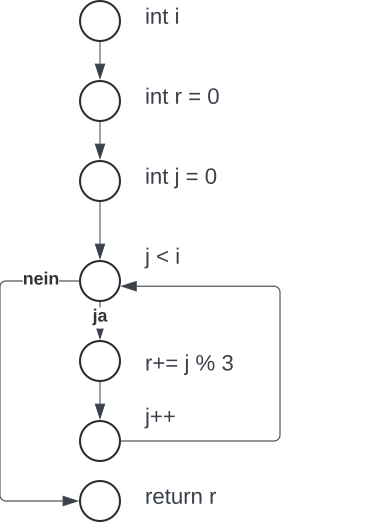
\includegraphics[scale=0.4]{part four/Werkzeuggestützte Analyse/img/kontrollflussgraph}
    \caption{Kontrollflussgraph für \textit{countVowels()}. (Quelle: in Anlehnung an \cite[Abb. 4.1, 32]{Wed09c})}
    \label{fig:kontrollflussgraph}
\end{figure}

\section{Datenflussanomalieanalyse und abstrakte Interpretation}
Es gitb auch Werkzeuge, die unabhängig von Mustern Fehlersituationen auch anhand der Analyse des Quelltextes erkennen können.\\
Hierzu gibt es zwei Verfahren, die \textbf{Datenflussanomalieanalyse} und die \textbf{abstrakte Interpretation}: Bei beiden Verfahren wird der Zugriff auf Variablen durch mögliche Programmabläufe untersucht (vgl.~\cite[33]{Wed09c}).


\subsection{Datenflussanomalieanalyse}
Die Abfolgen der \textbf{Zugriffe auf Variablen} in den verschiedenen Pfaden eines Kontrollflussgraphen werden bei der \textbf{Datenflussanomalieanalyse} analysiert.\\

\noindent
Zugriffe auf eine Variable werden dazu durch drei Attribute beschrieben (s. Tabelle~\ref{tab:dfaa}):


\begin{table}[]
    \centering
    \setlength{\tabcolsep}{0.5em}
    \def\arraystretch{1.5}
    \begin{tabular}{|c|l|l|}
        \hline
        \textbf{Kürzel} & \textbf{Bedeutung} & \textbf{Beispiel}                                            \\ \hline
        \textbf{d}                                                    & Definition                                                      & \code{x = 5}                                                          \\ \hline
        \textbf{r}                                                    & Referenzierung                                                  & \begin{tabular}[c]{@{}l@{}}\code{y = x + 1}\\ \code{if (x < 4)}\end{tabular} \\ \hline
        \textbf{u}                                                    & Undefinition                                                    & \code{int x;} oder Zerstörung                                         \\ \hline
    \end{tabular}
    \caption{Kürzel in der Datenflussanomalieanalyse und ihre Bedeutung. (Quelle: \cite[33]{VW16c})}
    \label{tab:dfaa}
\end{table}

\noindent
Die Abfolge von Attributen in einem Pfad wird als \textbf{Zugriffssequenz} bezeichnet.

\subsubsection*{Beispiel}

Sei folgendes Beispiel in Java gegeben:

\begin{minted}{java}
    class Pair {
        private int min;
        private int max;

        public void minMax() {
            int hilf;
            if (min > max) {
                max = hilf;
                max = min;
                hilf = min;
            }
        }
    }
\end{minted}

\noindent
\code{minMax()} soll überprüfen, ob \code{min} kleiner als \code{max}, und ansonsten den Inhalt beider vertauschen, was aber im Code nicht umgesetzt ist.
Der Code weist also einen Defekt auf.\\

\noindent
Der Kontrollflussgraph zu \code{minMax} ist in Abbildung~\ref{fig:minmax} gezeigt.

\begin{figure}
    \centering
    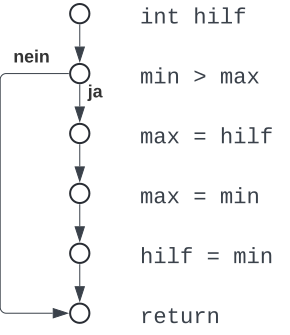
\includegraphics[scale=0.4]{part four/Werkzeuggestützte Analyse/img/minmax}
    \caption{Kontrollflussgraph für \textit{minMax()}. (Quelle: eigene)}
    \label{fig:minmax}
\end{figure}

\noindent
Für die \textit{zwei} möglichen Pfade (\code{min > max} / \code{min <= max}) sind die Zugriffssequenzen der 3 Variablen \code{min}, \code{max} und \code{hilf} in Tabelle~\ref{tab:minmax} aufgelistet.

\begin{table}[]
    \centering
    \setlength{\tabcolsep}{0.5em}
    \def\arraystretch{1.5}
    \begin{tabular}{|c|c|c|}
        \hline
         & \textbf{min > max} & \textbf{min <= max}\\
        \hline
        \code{hilf}                                           & \textbf{urdu}                                          & \textbf{uu}                  \\ \hline
        \code{max}                                            & \textbf{rdd}                                           & \textbf{r}                   \\ \hline
        \code{min}                                            & \textbf{rrr}                                           & \textbf{r}                   \\ \hline
    \end{tabular}
    \caption{Zugriffssequenzen der Variablen für zwei mögliche Pfade in \textit{minMax()}.}
    \label{tab:minmax}
\end{table}

\subsubsection*{3 mögliche Anomalien}
Es gibt bei der Datenflussanomalieanalyse \textbf{3 mögliche Anomalien}, die allesamt in Tabelle~\ref{tab:minmax} auftauchen:

\begin{itemize}
    \item \textbf{ur-Anomalie}: Zugriff auf eine Variable, bevor sie initialisiert wurde.\\
    Der Compiler von Java erkennt diesen Defekt.
    \item \textbf{du-Anomalie}: Definition einer Variable und anschließende Undefinition, ohne, dass auf sie davor lesend / schreibend verwendet wurde
    \item \textbf{dd-Anomalie}: Mehrmalige Definition einer Variable, ohne, dass zwischendurch lesend auf sie zugegriffen wird.
\end{itemize}

\subsubsection*{Anomalie ungleich Defekt}
\textit{Wedemann} stellt fest, dass die \textbf{ur-Anomalie} einen eindeutigen Defekt darstellt, während das bei der \textbf{dd-} bzw. \textbf{du-Anomalie} nicht so ist: Solche Anomalien können u.a. bei Schleifen auftreten (vgl.~\cite[35]{Wed09c}).

\subsubsection*{Schleifen}
Bei Code mit Schleifen ist die Anzahl der möglichen Pfade für eine vollständige Analyse meistens zu groß: Es reicht aber aus, den abweisenden Fall sowie zwei Durchläufe zu analysieren, da bei den Alternativen prinzipiell keine Anomalien hinzukommen können (vgl.~\cite[35]{Wed09c}).

\subsubsection*{Vorgehen}
Das Vorgehen zur Nutzung solcher Werkzeuge entspricht dem Vorgehen bei den bisher beschriebenen werkzeuggestützten Analyse (s. Abschnitt~\ref{sec:programmierrichtlinien}).
Eine sorgfältige Einweisung der Mitarbeiter ist wichtig.

\subsubsection*{Pro und Contra}
\textbf{ur-Anomalien} werden von vielen Compilern entdeckt.
Zur Entdeckung von \textbf{dd-} bzw. \textbf{du-Anomalien} gibt es nicht viele Werkzeuge\footnote{
für Java gibt es beispielsweise das bereits erwähnte \textit{PMD}, s. Abschnitt~\ref{sec:typische-defekte}
}.
Viele Werkzeuge beschränken sich außerdem auf die Analyse von lokalen Variablen und analysieren keine Instanzvariablen, weshalb der Einsatz der Datenflussanomalieanalyse in den meisten Bereichen nur für qualifizierte Entwickler mit einigen Einschränkungen möglich ist (vgl.~\cite[36]{Wed09c}).
Trotz alledem erlaubt die Datenflussanomalianalyse das Auffinden insb. von Defekten in Zusammenhang mit Schleifen, die sonst nur schwer zu entdecken gewesen wären.

\subsection{Abstrakte Interpretation}\label{subsec:abstrakte-interpretation}
Ähnlich wie bei der \textbf{Datenflussanomalieanalyse} wird bei der \textbf{abstrakten Interpretation} bzw. \textbf{abstrakten Semantik} die Nutzung von Variablen in allen Kontrollflüssen analysiert.\\
Es werden hierbei aber keine Kontrollflüsse \textit{konstruiert}, sondern es kommen aufwändige mathematische Verfahren zum Einsatz.

\subsubsection*{Analyse zugewiesener Werte}
Bei der \textbf{abstrakten Interpretation} wird nicht nur die Art der Nutzung von Variablen, sondern auch der Wert, der ihnen zugewiesen wird, analysiert.\\
\textit{Wedemann} gibt hierzu folgendes Beispiel an (vgl.~\cite[36]{Wed09c}):

\begin{minted}{java}
    public void f(int x) {
        if (x < 10) {
            for (int i = 0; i < x; i++) {
                if (i > 10) {
                    // nicht erreichbar
                }
            }
        }
    }
\end{minted}

\noindent
Zeile 5 ist nicht erreichbar:

\begin{enumerate}
    \item nach Zeile 2 is \code{x <= 9}
    \item nach jedem Schleifendurchlauf wird \code{i} um eins erhöht, bis \code{i == x} als Abbruchbedingung erfüllt ist.
    \item[] Da \code{x <= 9} als Voraussetzung gilt, kann also \code{i > 10} niemals erfüllt werden.
\end{enumerate}

\noindent
Analog wird bei der \textbf{abstrakten Interpretation} bspw. auf
\begin{itemize}
    \item die Überschreitung von Array-Grenzen
    \item Overflow bei skalaren Operationen
    \item Division durch 0
    \item Nutzung durch ungültige Zeiger (C / C++)
\end{itemize}
\noindent
geprüft.

\subsubsection*{Beweis der Abwesenheit von Laufzeitfehlern}
Werkzeuge sind auf diese Art und Weise also in der Lage für Quelltext anzugeben, wo prinzipiell keine Laufzeitfehler auftauchen, und wo sie sicher auftauchen werden.\\
Aus diesem Grund ist der Einsatz von solchen Werkzeugen bspw. im Automotive-Bereich vorgeschrieben (vgl.~\cite[36]{Wed09c}).\\
\textit{Wedemann} verweist ebenda auf \textit{Polyspace}\footnote{
\url{https://de.mathworks.com/products/polyspace.html}, abgerufen 24.05.2024
} als verbreitetes Werkzeug zur Analyse von C, C++ und Ada, merkt aber an, dass die Handhabung kompliziert ist und ein spezielles Training benötigt.

\section{Code-Metriken}
Eine andere Herangehensweise für die werkzeuggestützte Analyse stellt die Ermittlung von \textbf{Code-Metriken} dar.\\
Hierbei werden \textbf{Kennzahlen} bestimmt, anhand derer sich die \textbf{Wartbarkeit} von Source-Code beurteilen lässt.\\
Code-Metriken stehen in \textit{engem Zusammenhang} mit \textbf{Prinzipien guten Entwurfs} (s. Abschnitt~\ref{sec:prinzipien-guten-entwurfs}).\\
Im Folgenden werden die laut \textit{Wedemann} wichtigsten Code-Metriken zur Analyse objektorientierter Software vorgestellt (s. Abbildung~\ref{fig:metriken}).

\begin{figure}
    \centering
    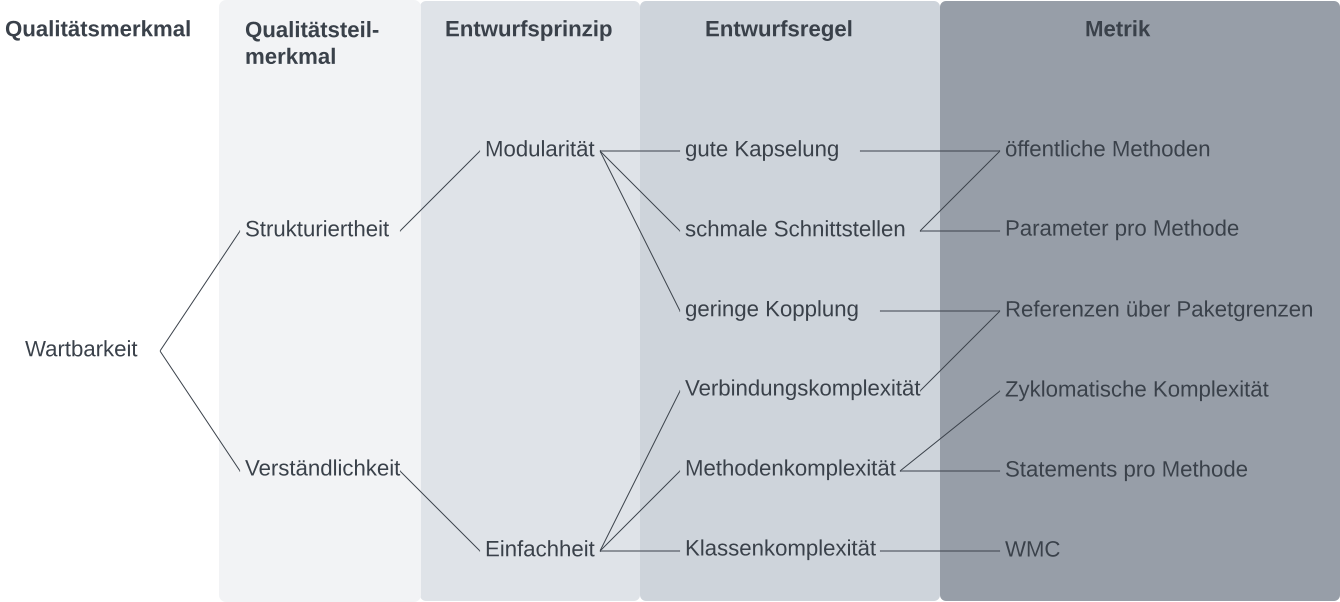
\includegraphics[scale=0.35]{part four/Werkzeuggestützte Analyse/img/metriken}
    \caption{Typische Metriken zur Bestimmung des \textbf{Qualitätsmerkmals} \textit{Wartbarkeit} und ihr Zusammenhang mit den Qualitätsteilmerkmalen. \textbf{WMC} steht für  \textit{Weighted Mean Complexity} (s. ``Komplexität``). (Quelle: in Anlehnung an \cite[Abb. 4.3, 37]{Wed09c})}
    \label{fig:metriken}
\end{figure}

\begin{tcolorbox}[colback=white]
    \textbf{Wartbarkeit} von Code ist immer auch abhängig von den Qualitätsteilmerkmalen \textbf{Strukturiertheit} und \textbf{Verständlichkeit}, die sich mit Metriken messen lassen.
\end{tcolorbox}
\vspace{2mm}

\noindent
Folgende Qualitätsteilmerkmale werden erfüllt, wenn der Entwurf bestimmte Regeln bzw. Prinzipien befolgt, die sich dann in der Implementierung widerspiegeln:

\begin{itemize}
    \item gut strukturierter Code ist leichter zu ändern
    \item einfach zu verstehender Code lässt sich leichter ändern
\end{itemize}

\begin{tcolorbox}
    Ob die Qualitätsforderung \textbf{Wartbarkeit} erreicht ist, kann auch durch Code-Metriken überprüft werden, die versuchen, Prinzipien wie \textbf{Modularität} und Regeln wie \textbf{geringe Kopplung} in Zahlen zu fassen (vgl.~\cite[38]{Wed09c}).
\end{tcolorbox}
\vspace{2mm}

\subsection*{Modularität}
Wenn Quellcode \textbf{modular} ist, ist er auch \textbf{gut strukturiert}.\\
Zur Messing von \textbf{Modularität} werden Metriken zu 3 \textbf{Entwurfsregeln} betrachtet:

\begin{enumerate}
    \item \textbf{gute Kapselung} entsteht durch \textit{wenige} \textbf{öffentliche Methoden}
    \item \textbf{schmale Schnittstellen} bewirkt eine \textbf{niedrige Kopplung}: Dies wird insgesamt erreicht durch \textit{wenig öffentliche Methoden} mit einer \textit{geringen Anzahl von Parametern}\footnote{
    s. auch \textit{Data Coupling}, Abschnitt~\ref{subsec:lose-kopplung}
    }
    \item \textbf{geringe Kopplung von Paketen} wird erreicht, indem wenige Referenzen über Paketgrenzen hinausgehen.
\end{enumerate}


\subsection*{Zyklomatische Zahl}
Zur Abschätzung der \textbf{Komplexität einer Methode} wird häufig die \textbf{zyklomatische Zahl} (auch: \textit{McCabe-Metrik}\footnote{
s. \url{https://de.wikipedia.org/wiki/McCabe-Metrik}, abgerufen 25.05.2024
}) verwendet.\\
Sie gibt die Anzahl unabhängiger Zyklen an, also die Anzahl der Verzweigungen in einer Methode $+1$.\\
Formal lässt sich die \textbf{zyklomatische Zahl} aus dem \textbf{Kontrollflussgraphen} bestimmen: Mit $n$ als Anzahl der Knoten und $e$ als Anzahl der Kanten berechnet sich die zyklomatische Zahl zu $Z = e - n + 2$.\\
Ist eine zyklomatische Zahl hoch, wird von einer hohen Komplexität ausgegangen.\\
Als Beispiel sei nochmals der Kontrollflussgraph zu der Methode \code{countVowels()}\footnote{
    s. Abschnitt~\ref{sec:hilfsmittel-kontrollflussgraph}
} gegeben (s. Abbildung~\ref{fig:zyklomatischezahl}):  Mit $n = 8$ und $e = 9$ berechnet sich die zyklomatische Zahl zu $e - n + 2 = 9 - 8 + 2 = 3$


\begin{figure}
    \centering
    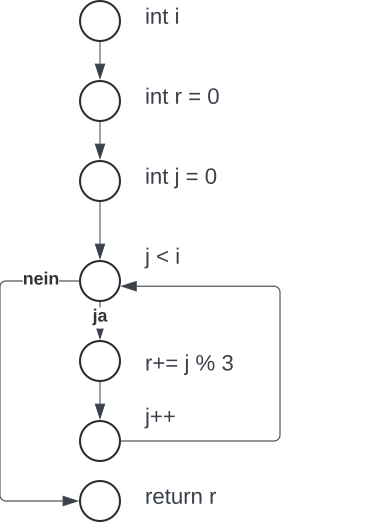
\includegraphics[scale=0.4]{part four/Werkzeuggestützte Analyse/img/kontrollflussgraph}
    \caption{Kontrollflussgraph für \textit{countVowels()}, für den sich eine zyklomatische Zahl von $Z=3$ ergibt. (Quelle: in Anlehnung an \cite[Abb. 4.1, 32]{Wed09c})}
    \label{fig:zyklomatischezahl}
\end{figure}

\noindent
\textit{Wedemann} merkt an, dass die zyklomatische Zahl von zwei \textit{verschachtelten} Schleifen oder Bedingungen genauso groß sei wie die von zwei aufeinanderfolgenden Schleifen oder Bedingungen, obwohl verschachtelte Konstrukte meist schwerer verständlich sind, und dass eine zyklomatische Zahl von $>10$ von vielen Autoren als problematisch betrachtet wird\footnote{
McCabe verwendet in seinem Paper $10$ als ``a reasonable, but not magical,  upper limit.`` (\cite[314]{McC76})
} (vgl.~\cite[38]{Wed09c}).


\subsection*{Komplexität}
Ein weiteres Maß für die \textbf{Komplexität einer Methode} ist die \textbf{Anzahl der Anweisungen}\footnote{auch: Anzahl der Zeilen. Eine Anweisung kann über mehrere Zeilen gehen.}.
Lange Methoden sind sicherlich schwieriger zu verstehen, weshalb auch hier weniger Anweisungen besser sind.\\
Die \textbf{Komplexität einer Klasse} kann mit Hilfe der \textbf{Weighted Mean Complexity} (\textit{WMC}) gemessen werden, für deren Bestimmung die zyklomatische Zahlen \textit{aller Methoden} zusammengezählt werden - auch hier ist ein geringerer Wert besser.

\subsection*{Vorgehen}
Für den Umgang mit den berechneten Zahlenwerten gibt es zwei Strategien:

\begin{enumerate}
    \item Zu den verschiedenen Metriken sind in der Literatur oder den Werkzeugen typische Grenzen angegeben, innerhalb derer Code als ``gut`` betrachtet werden kann.
    \item Da die in (1) erwähnten Grenzen willkürlich erscheinen können bzw. sich verschiedene Quellen bei der Angabe der Grenzen widersprechen können, werden Projekte oft mit einem Satz von Standardwerten untersucht und dann ggf. an das Projekt angepasst.
\end{enumerate}

\noindent
Werden Metriken in einem bereits fortgeschrittenen Projekt eingesetzt, sollten nur die Klassen und Methoden untersucht werden, die besonders auffällig sind.

\subsection*{Werkzeuge}
Für Java gibt es bspw. \textit{Metrics}\footnote{
\url{https://metrics.dropwizard.io}, abgerufen 25.05.2024
}, für PHP bspw. \textit{PHPMetrics}\footnote{
    \url{https://www.phpmetrics.org}, abgerufen 25.05.2024
}.

\subsection*{Pro und Contra}
Code-Metriken sind ein bewährtes Mittel zur Analyse von Code in Bezug auf \textbf{Wartbarkeit}.\\
Wenn Metriken parallel zur laufenden Entwicklung eingesetzt werden, können viele Schwachstellen vermieden werden - sie sind allerdings auch geeignet, um in fremden Code Schwachstellen zu entdecken, wodurch sie ein wertvolles Werkzeug für Projektleiter, QS-Verantwortliche und auch Kunden sind (vgl.~\cite[39]{Wed09c}).\\
In der Praxis kann es sich als schwierig erweisen, geeignete Metriken auszuwählen und die ermittelten Daten korrekt zu interpretieren: Hier werden fehlerhafte Ergebnisse dann durch ungeeignete oder falsch interpretierte Metriken verursacht, was zu Ablehnung der Werkzeuge führen kann.\\
Es ist also ratsam, sich in die einzusetzenden Metriken einzuarbeiten und an bekannten Projekten zunächst auszuprobieren.

\newpage
\section{Zusammenfassung}

\begin{itemize}
    \item Anforderungen lassen sich bei Projekten vorab nicht genügend festlegen.
    \item Fehlt im Team die Erfahrung oder werden neue Technologien eingesetzt, ist ein ausgereifter Entwurf nicht machbar.
    \item Bei großen Projekten würde man unter diesen Voraussetzungen mit dem Wasserfallmodell nicht flexibel genug sein,
    um auf Änderungen reagieren zu können.
    \item Aus diesem Grund gibt es alternative Modelle, die eingesetzt werden können:
        \begin{itemize}
            \item \textbf{inkrementell}: Aufteilung der Anforderungen, so dass Teilsysteme umgesetzt und an den Kunden ausgeliefert werden können
            Die Teilsysteme werden sequentiell bearbeitet.
            \item \textbf{iterativ}: In Iterationen wird das Projekt in Zeitabschnitte unterteilt, in denen die Anforderungen umgesetzt werden; entsprechend dem Spiralmodell zunächst die risikoreichsten.
            Vorhergehende Ergebnisse werden in darauffolgenden Iterationen weiterbearbeitet.
            Ein bekanntes iteratives Modell ist \textit{RUP}, bei dem einzelne Phasen Ergebnis-Artefakte liefern, wie Anwendungsfälle oder Klassendiagramme.
            \item \textbf{nebenläufig}: Die Aufgaben werden aufgeteilt in parallel (oder nacheinander) bearbeitbare Aufgaben, die dann von den Mitarbeitern umgesetzt werden.
        \end{itemize}
    \item Die genannten Modelle werden häufig nicht isoliert betrachtet, sondern je nach Projekt auch kombiniert, insb. bei dem \textbf{agilen Vorgehen}.
\end{itemize}



